%%%%%%%% ICML 2022 EXAMPLE LATEX SUBMISSION FILE %%%%%%%%%%%%%%%%%

\documentclass[nohyperref]{article}

% Recommended, but optional, packages for figures and better typesetting:
\usepackage{microtype}
\usepackage{graphicx}
\usepackage{subfigure}
\usepackage{booktabs} % for professional tables

% hyperref makes hyperlinks in the resulting PDF.
% If your build breaks (sometimes temporarily if a hyperlink spans a page)
% please comment out the following usepackage line and replace
% \usepackage{icml2022} with \usepackage[nohyperref]{icml2022} above.
\usepackage{hyperref}

% Attempt to make hyperref and algorithmic work together better:
\newcommand{\theHalgorithm}{\arabic{algorithm}}

% Use the following line for the initial blind version submitted for review:
% \usepackage{icml2022}
\usepackage[accepted]{icml2022}

% For theorems and such
\usepackage{amsmath}
\usepackage{amssymb}
\usepackage{mathtools}
\usepackage{amsthm}
\usepackage{bm}

% if you use cleveref..
\usepackage[capitalize,noabbrev]{cleveref}

%%%%%%%%%%%%%%%%%%%%%%%%%%%%%%%%
% THEOREMS
%%%%%%%%%%%%%%%%%%%%%%%%%%%%%%%%
\theoremstyle{plain}
\newtheorem{theorem}{Theorem}[section]
\newtheorem{proposition}[theorem]{Proposition}
\newtheorem{lemma}[theorem]{Lemma}
\newtheorem{corollary}[theorem]{Corollary}
\theoremstyle{definition}
\newtheorem{definition}[theorem]{Definition}
\newtheorem{assumption}[theorem]{Assumption}
\theoremstyle{remark}
\newtheorem{remark}[theorem]{Remark}

% Todonotes is useful during development; simply uncomment the next line
%    and comment out the line below the next line to turn off comments
%\usepackage[disable,textsize=tiny]{todonotes}
\usepackage[textsize=tiny]{todonotes}

% custom packages & commands
% \input{command_math}
% \usepackage{algorithm}
% \usepackage[noend]{algorithmic}

\newcommand\rurl[1]{\href{http://#1}{\nolinkurl{#1}}}
\newcommand{\globalTitle}{Self-Supervision is All You Need for Solving Rubik's Cube}
\usepackage{titlesec}
\usepackage[para]{footmisc}


% The \icmltitle you define below is probably too long as a header.
% Therefore, a short form for the running title is supplied here:
% \icmltitlerunning{Submission and Formatting Instructions for ICML 2022}
\icmltitlerunning{\globalTitle}

\begin{document}

\twocolumn[
% \icmltitle{Submission and Formatting Instructions for \\
%           International Conference on Machine Learning (ICML 2022)}
\icmltitle{\globalTitle}

% It is OKAY to include author information, even for blind
% submissions: the style file will automatically remove it for you
% unless you've provided the [accepted] option to the icml2022
% package.

% List of affiliations: The first argument should be a (short)
% identifier you will use later to specify author affiliations
% Academic affiliations should list Department, University, City, Region, Country
% Industry affiliations should list Company, City, Region, Country

% You can specify symbols, otherwise they are numbered in order.
% Ideally, you should not use this facility. Affiliations will be numbered
% in order of appearance and this is the preferred way.
\icmlsetsymbol{equal}{}

\begin{icmlauthorlist}
% \icmlauthor{Firstname1 Lastname1}{equal,yyy}
% \icmlauthor{Firstname2 Lastname2}{equal,yyy,comp}
% \icmlauthor{Firstname3 Lastname3}{comp}
% \icmlauthor{Firstname4 Lastname4}{sch}
% \icmlauthor{Firstname5 Lastname5}{yyy}
% \icmlauthor{Firstname6 Lastname6}{sch,yyy,comp}
% \icmlauthor{Firstname7 Lastname7}{comp}
% %\icmlauthor{}{sch}
% \icmlauthor{Firstname8 Lastname8}{sch}
% \icmlauthor{Firstname8 Lastname8}{yyy,comp}
% %\icmlauthor{}{sch}
% %\icmlauthor{}{sch}
\icmlauthor{Kyo Takano}{na}
\end{icmlauthorlist}

% \icmlaffiliation{yyy}{Department of XXX, University of YYY, Location, Country}
% \icmlaffiliation{comp}{Company Name, Location, Country}
% \icmlaffiliation{sch}{School of ZZZ, Institute of WWW, Location, Country}
\icmlaffiliation{na}{Tokyo, Japan}

% \icmlcorrespondingauthor{Firstname1 Lastname1}{first1.last1@xxx.edu}
% \icmlcorrespondingauthor{Firstname2 Lastname2}{first2.last2@www.uk}
\icmlcorrespondingauthor{}{kyo.takano@mentalese.co}

% You may provide any keywords that you
% find helpful for describing your paper; these are used to populate
% the "keywords" metadata in the PDF but will not be shown in the document
% \icmlkeywords{Machine Learning, ICML}
\icmlkeywords{Rubik's Cube, pathfinding, combinatorial search, self-supervised learning}
\vskip 0.3in
]

% this must go after the closing bracket ] following \twocolumn[ ...

% This command actually creates the footnote in the first column
% listing the affiliations and the copyright notice.
% The command takes one argument, which is text to display at the start of the footnote.
% The \icmlEqualContribution command is standard text for equal contribution.
% Remove it (just {}) if you do not need this facility.

\printAffiliationsAndNotice{}  % leave blank if no need to mention equal contribution
% \printAffiliationsAndNotice{\icmlEqualContribution} % otherwise use the standard text.

\begin{abstract}
    Existing combinatorial search methods are often complex and require some expertise.
    In this work, we propose a simple and performant deep learning method, especially for goal-predefined combinatorial problems represented by Rubik's Cube.
    We show that, for solving such problems with high optimality, it can be sufficient to train a deep neural network on random scrambles branching from the goal state.
    When tested on Rubik's Cube, our method outperformed the previous state-of-the-art method DeepCubeA in solution optimality, being 10 times more efficient in training and 2.0 times in inference.
    One key assumption is that, when viewed from scrambled states, random moves from the goal are biased to be optimal.
    We also demonstrate the proposed method on 15 Puzzle and Lights Out.
\end{abstract}

\begin{figure}[h!]
    \centering
    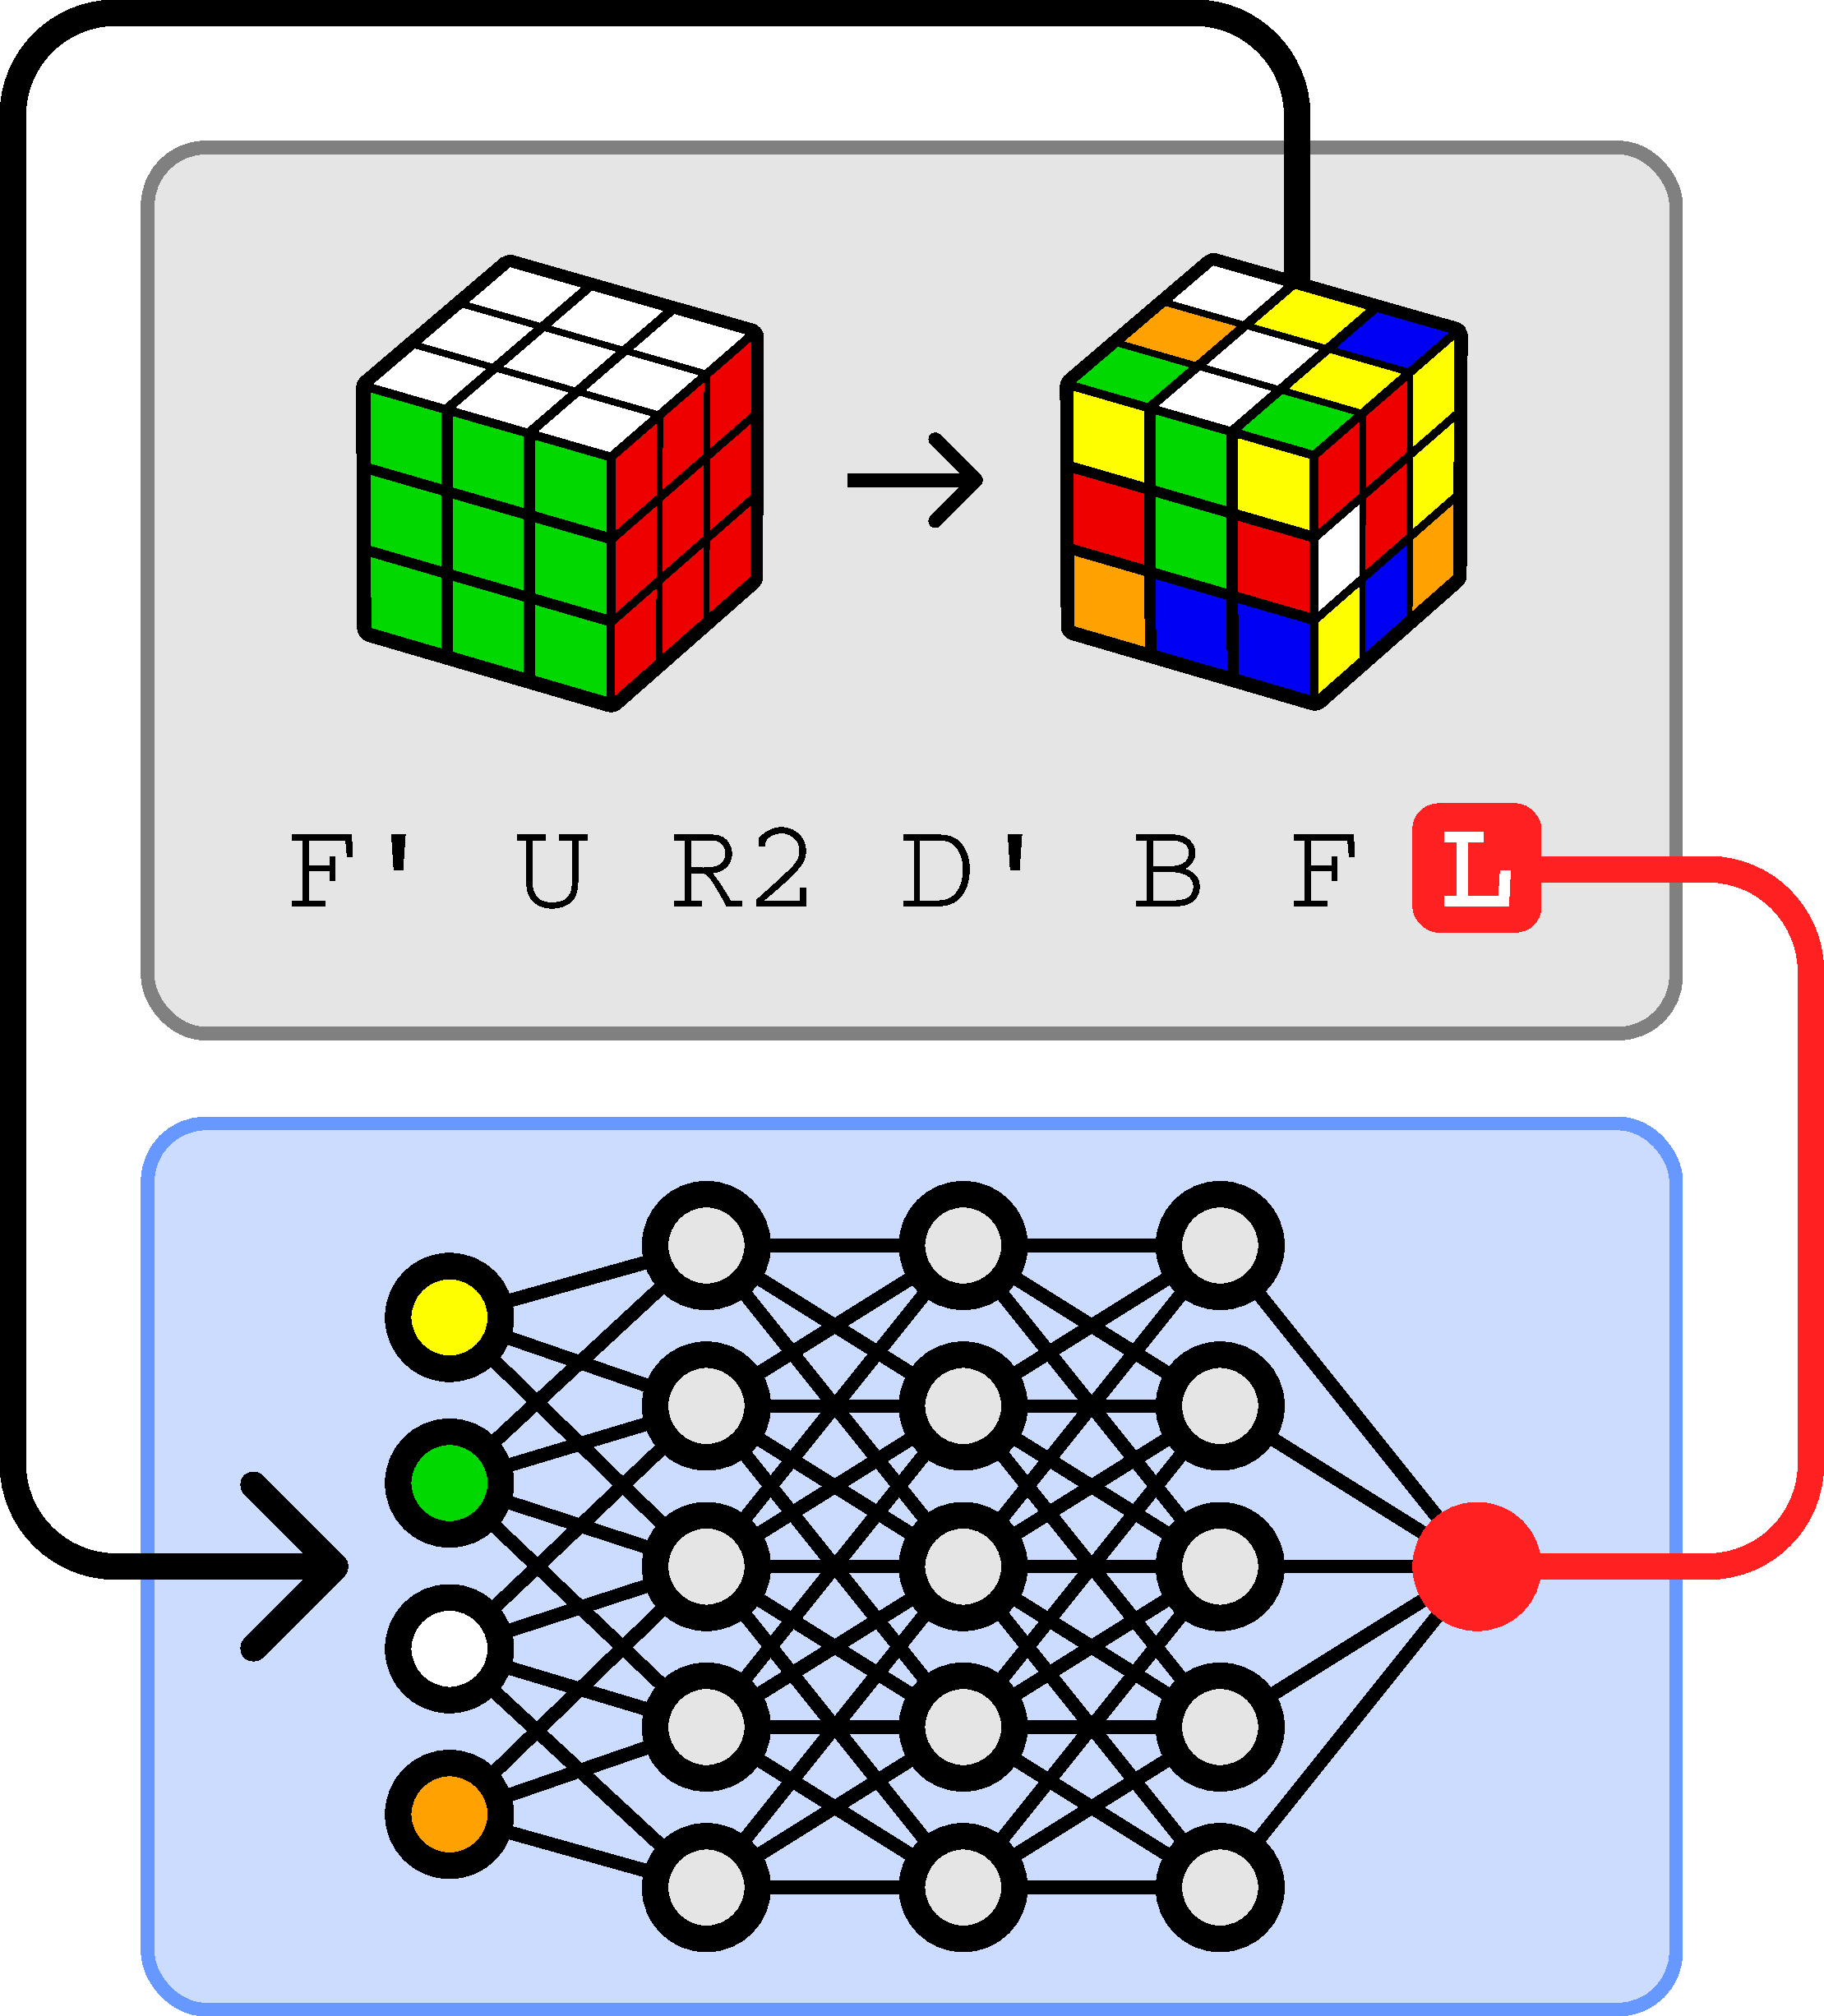
\includegraphics[width=0.598290598\columnwidth]{figures/overview.pdf}
    \caption{
        All you need for training a Deep Neural Network (DNN) to solve Rubik's Cube.
        We apply a sequence of random moves to the goal state, and at each step, the DNN learns to predict the last move of the scramble based on the resulting state.
        We assume that, although random, the scramble moves are biased to be optimal.
        When solving, we can explore a solution simply by inverting moves inferred by the DNN.
    }
    \label{fig:overview}
\end{figure}

\section{Introduction}
Combinatorial search is important both in theory and practice.
One representative example is \textit{Traveling Salesman Problem}, in which a salesman tries to travel through multiple cities in the shortest path possible~\citep{applegate2011traveling, russell2021artificial}.
Despite how easy it sounds, due to its combinatorial complexity, the problem is labeled \textit{NP-hard}~\citep{papadimitriou1998combinatorial}; as the number of cities grows, the number of possible combinations to search for explodes, easily exceeding the limits of a classical computer.
In the real world, algorithms for such problems have many applications including planning, scheduling, resource allocation, route planning, and so on.

Since the naive brute-force search is impractical, past researchers have developed several search methods to address the complexity of such problems.
These include exact algorithms to systematically find an optimal solution within an acceptable amount of time, and heuristic algorithms to find a good enough solution faster.
Most recently, deep learning has emerged as a method for automatically training a heuristic function that is optimized for a given objective.
Deep reinforcement learning, in particular, has enabled automatic training of a Deep Neural Network (DNN) as such to solve a combinatorial problem near-optimally, even without labeled data or a huge memory~\citep{mazyavkina2021reinforcement,vesselinova2020learning}.
By rewarding efficient moves/actions, a DNN can learn to find increasingly better solutions.

Nevertheless, combinatorial search is still no easy task.
Implementing an explicit search algorithm often requires not only expertise in the area but also commensurate computational resources and human efforts.
Meanwhile, reinforcement learning may be useful for automating part of that process, but it still requires familiarity with the method itself and a lot of trial and error.

In the present study, taking \textit{Rubik's Cube} as a particular example, we focus on a specific class of combinatorial problems---namely, those with a predefined goal---and propose a novel method for solving such problems.
The idea is straightforward:
train a DNN on mere random scrambles diverging from the goal, as depicted in Figure~\ref{fig:overview}.
We evaluate our method against the previous state-of-the-art deep learning method named DeepCubeA~\citep{agostinelli2019solving}, by experimenting with Rubik's Cube.

\section{Related Work}
Rubik's Cube and 15 Puzzle are typical examples of goal-predefined combinatorial problems.
To generalize, the task in such problems is to find a sequence of moves that reaches the predefined goal from a given state.
For individual descriptions, see Experiment for Rubik's Cube and Appendix~\ref{appendix:15} for 15 Puzzle.
Henceforth, we consider any of such problems as a pathfinding task on an \textit{implicit} graph.
Each node in the graph represents a unique state, and edges indicate moves to its adjacent nodes with equal probability.

Among various methods for solving those problems, we pay particular attention to two leading methods with highly optimality.
First, Iterative Deepening A* (IDA*), a complete search algorithm that is guaranteed to find an optimal solution in a reasonable time~\citep{korf1985depth,korf1997finding}.
Second, DeepCubeA, a near-optimal method that leverages deep reinforcement learning~\citep{agostinelli2019solving}.
Both are forward search methods to find the goal by expanding nodes from a given state, in order of their estimated distances.

\citet{korf1985depth} developed IDA* as the first admissible search algorithm to solve 15 Puzzle optimally.
IDA* is a combination of two algorithms: \underline{I}terative \underline{D}eepening Depth-First Search (IDDFS) and \underline{A*} search~\citep{hart1968formal}.
IDDFS is a depth-first search that iteratively deepens until a solution is found, and like a breadth-first search, it is guaranteed to find optimal solutions.
However, if a state space is too large, the search algorithm becomes infeasible to run within a realistic time frame.
To enable IDDFS in such a vast state space, \citet{korf1985depth} incorporated the idea of A* search, which expands nodes in order of their estimated total distance formulated as
\begin{equation}
    f(x) = g(x)+h(x)
    \label{eq:astar}
\end{equation}
where $x$ is an expanded node, $g(x)$ is the depth from the starting node, and $h(x)$ is the \textit{lower bound} of the remaining distance to the goal informed by theory heuristic.
Using the same formula, IDA* iteratively increases the threshold for $f(x)$ instead of depth, greatly reducing the number of expanded nodes without compromising the optimality.
Later, Korf extended IDA* as the first optimal solver against Rubik's Cube, incorporating a pattern database that precomputes lower bounds of distances corresponding to particular patterns (1997).
Since then, more efficient implementations have followed this approach~\citep{korf2008linear,arfaee2011learning,rokicki2014diameter}.
Even so, they remain problem-specific and require domain knowledge of group theory and search.

DeepCube was the first to formulate Rubik's Cube as a reinforcement learning task and to solve it successfully~\citep{mcaleer2018solving}, which soon evolved as DeepCubeA with significant performance improvement~\citep{agostinelli2019solving}.
DeepCubeA trains a DNN in place of $h(x)$ in Eq.~\ref{eq:astar} to estimate the distance from a given state to the predefined goal.
By relatively discounting $g(x)$ like weighted A*~\citep{pohl1970heuristic, ebendt2009weighted} and expanding a certain number of nodes per iteration, DeepCubeA then searches for a solution so that the approximate lower bound of total distance $f(x)$ is as small as possible.
DeepCubeA is also shown applicable to similar problems like 15 Puzzle and its variants, as well as Lights Out and Sokoban~\citep{agostinelli2019solving}.

Unlike IDA*, which relies on group theory, DeepCubeA automatically trains a DNN as a function approximator to estimate distances.
The use of DNN is well suited for this task for a few reasons.
First, it can learn complex patterns in data using a fixed number of parameters.
Next, it also generalizes well to cases not seen during training.
These features are especially convenient when a state space is too large to exhaustively traverse and store in memory.
Still, however, deep reinforcement learning is inherently complex and unstable, requiring careful design and hyperparameter tuning.
In DeepCubeA, \citet{agostinelli2019solving} had to check regularly that the training loss falls below a certain threshold before saving the DNN, to avoid local optima and performance degradation.

While both methods are powerful, they still require complex implementation with specialized knowledge.
Instead of estimating the distance to guide a search, we propose a more direct method to infer the path itself.
Our method trains a DNN on backward scrambles from the goal, treating them as inverse solutions from the resulting states.

\vspace{-1.2mm}
\section{Proposed Method}
A goal-predefined combinatorial problem can also be regarded as the task of tracing a scramble back to the goal.
Although the actual scramble is unobservable, it may still be possible to infer a plausible scramble as leading up to a given state.
Desirably, such a scramble should be as short as possible.
To this end, we propose a simple deep learning method to infer a scramble as a backward solution, one move at a time from a given state.

When training a DNN, our method sequentially scrambles the target problem from its goal state with random moves.
At each step of the scramble, the DNN learns to predict the last move of the scramble up to that point, based on the resulting state.
Algorithm~\ref{alg:training} provides the pseudocode of the training process, and Figure~\ref{fig:overview} captures an example data point on Rubik's Cube.
At inference, we search for a solution as a path back to the goal by repeatedly inverting moves that seemingly caused current states.
The core assumption is that the distribution of random scramble moves to be learned by a DNN is biased toward optimality, which we discuss in more detail below.
The miniature example in Figure~\ref{fig:miniature} illustrates how our method would work during both training and inference.

\begin{algorithm}[tb]
    \caption{The proposed algorithm to train a DNN using random scrambles.}
    \label{alg:training}
    \begin{algorithmic}
        \STATE {\bfseries Input:}
        \STATE
        \begin{tabular}{c@{}c@{\hskip 0.5em}l}
            \hspace{2.0em}$G$          & : & Goal state                     \\
            \hspace{2.0em}$\mathbb{M}$ & : & Set of moves                   \\
            \hspace{2.0em}$B$          & : & Number of scrambles in a batch \\
            \hspace{2.0em}$N$          & : & Number of moves in a scramble  \\
            \hspace{2.0em}$f_{\theta}$ & : & DNN parameterized by $\theta$  \\
        \end{tabular}
        \STATE {\bfseries Output:}\hspace{2.0em}$f_{\theta}$: Trained DNN
        \WHILE{not converged}
        \STATE $T \gets \varnothing$
        \FOR{$b=1$ {\bfseries to} $B$}
        \STATE $S \gets G$
        \FOR{$n=1$ {\bfseries to} $N$}
        \STATE $\textnormal{m} \gets$ random($\mathbb{M}$)
        \STATE $S \gets S \circ \textnormal{m}$
        \STATE $T \gets T \cup \{(S, \textnormal{m})\}$
        \ENDFOR
        \ENDFOR
        \STATE Update $f_{\theta}: S\mapsto \textnormal{m}$ using $T$
        \ENDWHILE
    \end{algorithmic}
\end{algorithm}



\begin{figure}[tb]
    \centering
    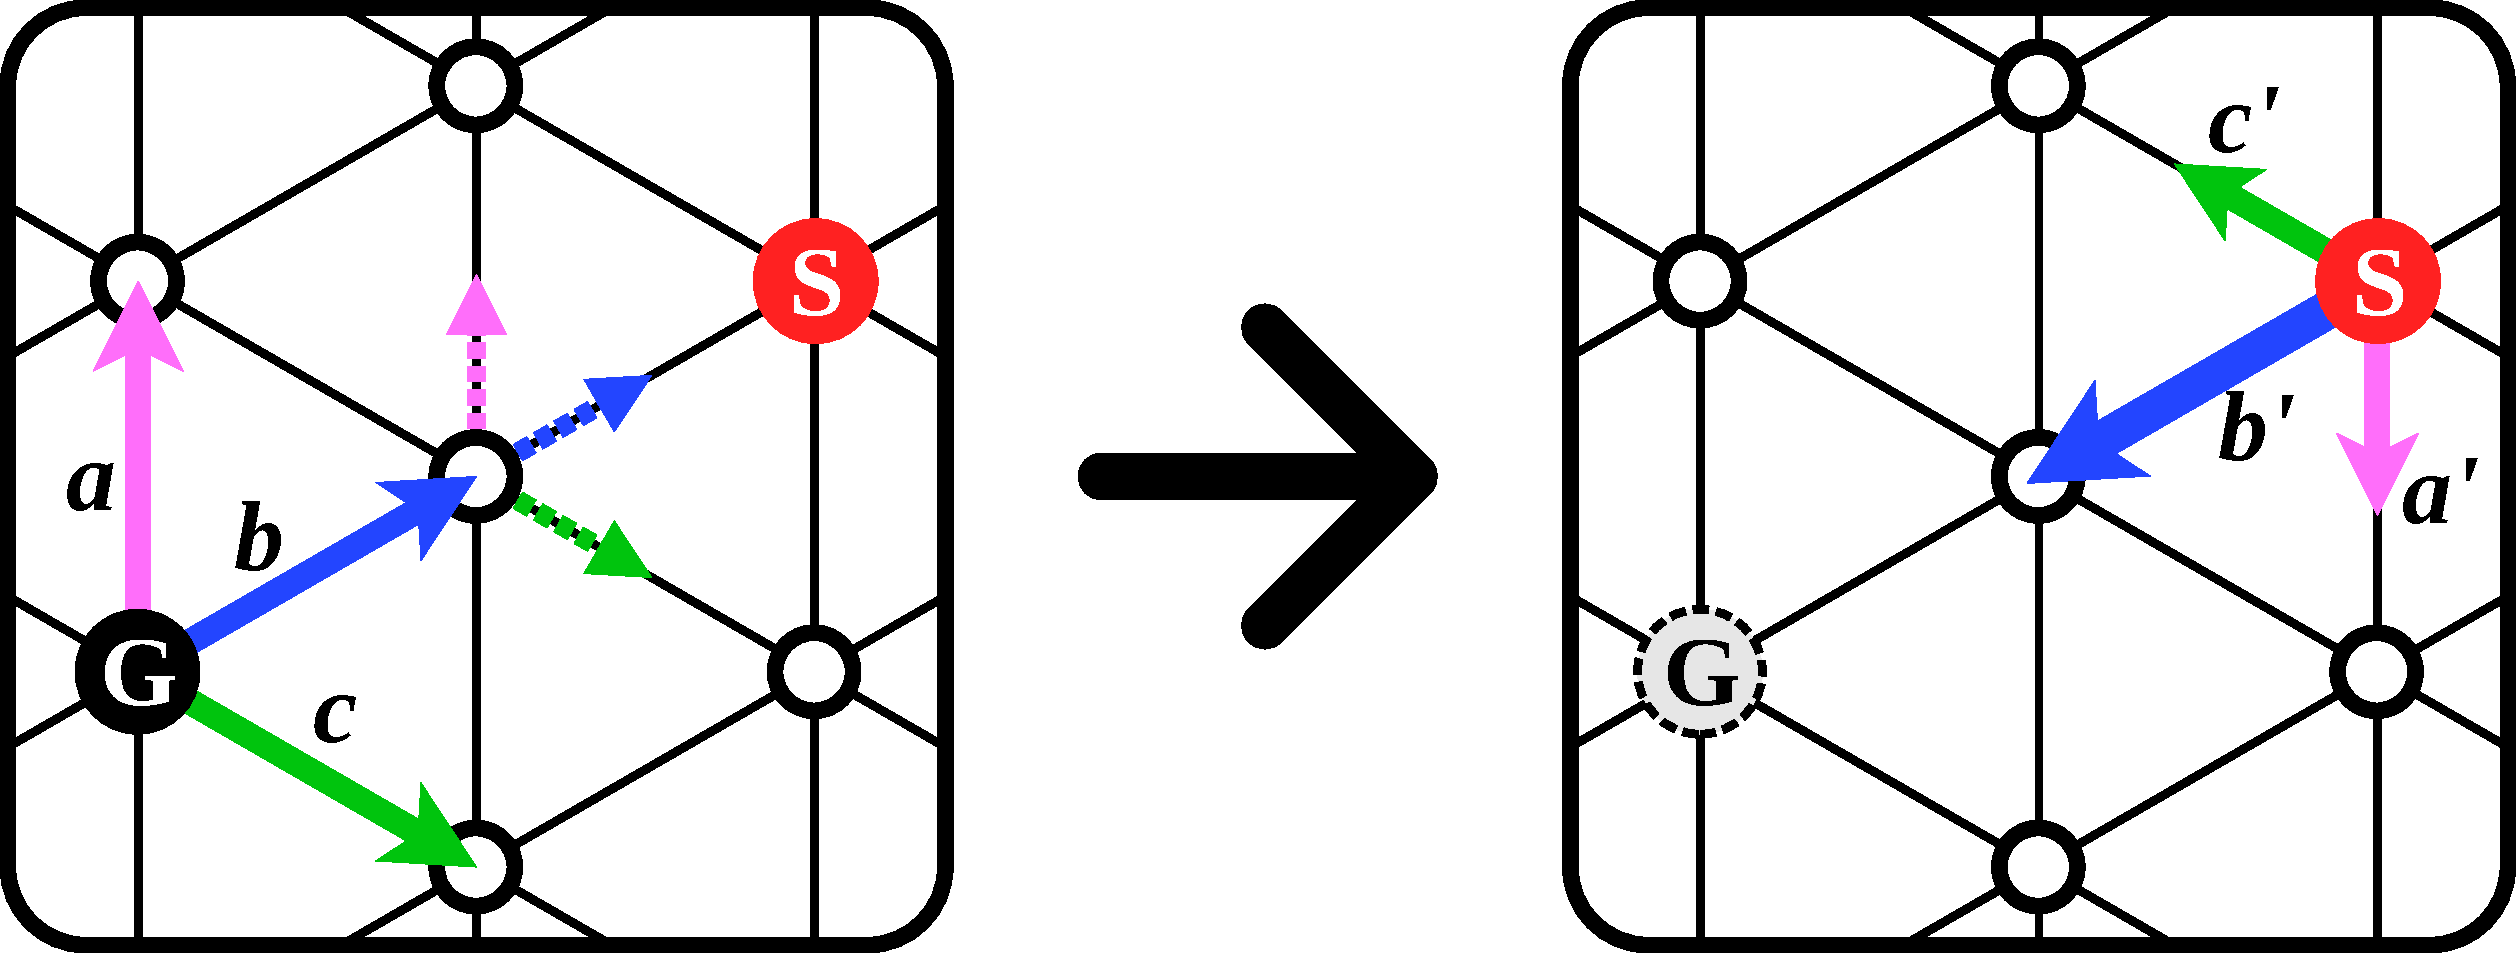
\includegraphics[width=1.0\columnwidth]{figures/method.example.pdf}
    \vspace{-1em}
    \caption{
        A miniature instance of combinatorial search with a predefined goal.
        When random paths connect two nodes/states, the distribution of moves can be biased toward optimality.
        $Left$:
        Suppose that during training, random moves $\{\bm{a}, \bm{b}, \bm{c}\}$ can occur at each node with an equal probability of $1/3$ and a combination of these moves generates an unknown path between nodes \textbf{G} (\underline{G}oal) and \textbf{S} (\underline{S}cramble).
        Adding up the probabilities of all the possible paths at each edge, we find that moves appearing on shorter paths are more likely to comprise the path of interest.
        A DNN can internalize this distribution by learning the state-to-move mapping, assuming that every state has a unique state pattern.
        $Right$:
        At inference time, the DNN can find the optimal path from \textbf{S} to \textbf{G} by traversing back through the learned distribution, where optimal moves are more frequent than suboptimal ones.
        In this instance, $\bm{b'}$ would be predicted as optimal over the other inverse moves $\bm{a'}$ and $\bm{c'}$, both at \textbf{S} and its subsequent node.
    }
    \label{fig:miniature}
    \vspace{-2mm}
\end{figure}


\subsection{Assumptions}
Our method has two assumptions, which are not strictly necessary but are preferably satisfied by the target problem.
Assumption 1 concerns the performance limit of the resulting DNN, while Assumption 2 affects its learning efficiency.

\paragraph{Assumption 1.}
When random paths connect two nodes,
more optimal moves are more often the first move.\\
\\
Here, we base the optimality of a move on that of paths starting with it.
With respect to the optimality of \textit{paths}, obviously, the shorter a path between two nodes, the more likely it is to occur as a sequence of random moves.
At some nodes, however, many suboptimal paths may stack up on a particular edge, causing the corresponding move to be sampled more often than the optimal alternative(s).
Because we want to predict one move at a time, we need to discuss the optimality of moves at the node level.

Accordingly, we formulate the statistical condition under which Assumption 1 is true for a given problem.
Suppose that we have an unknown path connecting two nodes, where each possible move in $\mathbb{M}$ has an equal probability at all nodes.
Let $p_{N,\bm{a}}$ be the probability of a particular move $\bm{a} \in \mathbb{M}$ being the \textit{first} move of potential paths consisting of $N$ moves or more,
\begin{equation}
    p_{N,\bm{a}}=\sum_{k=N}^{k_{max}}\frac{C_{k|\bm{a}}}{|\mathbb{M}|^{k}}
    \label{eq:equation_1}
\end{equation}
where $k$ is the move count to the target node, $k_{max}$ is the maximum move count from the goal, $|\mathbb{M}|$ is the number of possible moves at each node, and $C_{k|\bm{a}}$ is the number of $k$-move paths starting with the move $\bm{a}$.
Likewise, let $\bm{b} \in \mathbb{M}$ be an alternative to $\bm{a}$ that results in paths consisting of at fewest $N+1$ moves, Assumption 1 can be formulated as $p_{N+1,\bm{b}}\leq p_{N,\bm{a}}$.
Provided that $p_{N,\bm{a}}=\sum_{N+1}^{k_{max}}(C_{k|\bm{a}}/|\mathbb{M}|^{k})+(C_{N|\bm{a}}/|\mathbb{M}|^N)$, it is equivalent to
\begin{equation}
    \sum_{k=N+1}^{k_{max}}\frac{C_{k|\bm{b}}}{|\mathbb{M}|^{k}}
    \leq
    \sum_{k=N+1}^{k_{max}}\frac{C_{k|\bm{a}}}{|\mathbb{M}|^{k}}+\frac{C_{N|\bm{a}}}{|\mathbb{M}|^N}
    \label{eq:equation_2}
\end{equation}
At this point, note that Eq.~\ref{eq:equation_2} cannot be proven always true.
This is simply because there can be paths in which moves violate this, and also because that depends on the implicit graph of the problem at hand.
Both $C_{k|\bm{a}}$ and $C_{k|\bm{b}}$ can be determined only through actual computation on specific paths of a specific problem, so the $\sum$ terms do not necessarily equal when paths start with different moves.
However, we can still assume the \textit{rough} equivalence of these $\sum$ terms and thus the \textit{tendency} that Eq.~\ref{eq:equation_2} stands.
For it to be false, there must be sufficiently more paths starting with the suboptimal move $\bm{b}$ than $\bm{a}$ to cumulatively cancel the remaining term ${C_{N|\bm{a}}}/{|\mathbb{M}|^N}$.
Thus, when sampling a random move, we assume that it tends to be optimal as comprising a path to the resulting state.

For the performance of the trained DNN, the target problem should preferably satisfy Assumption 1 as much as possible.
In Appendix~\ref{appendix:mini}, we test Assumption 1 on 2$\times$2$\times$2 Rubik's Cube by exhausting all possible scramble paths and show that more optimal moves are sampled more often.

\paragraph{Assumption 2.}
God's Number, the smallest number of moves sufficient to solve any state, or its estimate is known.\\
\\
The training data is generated by scrambling the problem from $1$ to $N$ times from its goal state.
Let $N_{G}$ be God's Number for a given problem.
If $N < N_{G}$, then the trained DNN would not generalize well to states of higher complexities that take $N+1$ moves or more, leading to poor performance at inference.
Conversely, overestimating $N_{G}$ may result in redundant moves being applied to the highest complexity states, likely adding unnecessary noise to the training data.

If this number is unknown or not even estimated, it may help to iteratively increase the scramble length as long as the DNN can learn to make predictions for maximally scrambled cases better than chance.
Under Assumption 1, such predictability suggests $N \approx N_{G}$, where $N$ is insufficient or just sufficient to fully scramble the problem within the diameter of its state space.

\vspace{-0.4em}
\section{Experiment}\label{sec:experiment}
To evaluate our method against DeepCubeA~\citep{agostinelli2019solving}, we employ the same problem setting and representation, dataset, and model architecture. After solving test cases, we compare our result to the published result of DeepCubeA and its update provided on GitHub\footnote{\rurl{github.com/forestagostinelli/DeepCubeA/}}.

\vspace{-0.1em}
\subsection{Rubik's Cube}
Rubik's Cube is a cubic puzzle with $6$ faces each having $9$ color stickers.
The goal is to move the stickers by rotating $6$ faces so that each has stickers of only a single color.
Including the goal state, the puzzle can have roughly $4.3\times 10^{19}$ different states.
As a combinatorial problem, solving the puzzle optimally is proven to be \textit{NP-complete}~\citep{demaine2018solving}.

We represent Rubik's Cube as a $324$-$D$ vector by assigning an index to every color at every sticker location ($6$ colors $\times 54$ sticker positions).
Also, to manipulate states, we use the quarter-turn metric (a 90° turn of a face counts as one move, whereas a 180° turn counts as two), meaning $12$ possible moves for any state.
In the notation, \texttt{U}, \texttt{D}, \texttt{L}, \texttt{R}, \texttt{B}, and \texttt{F} respectively denote a 90° clockwise turn on \textbf{U}p, \textbf{D}own, \textbf{L}eft, \textbf{R}ight, \textbf{B}ack, and \textbf{F}ront faces on the puzzle; if followed by a prime (\texttt{'}), counterclockwise.

\vspace{-0.1em}
\subsection{Dataset}
We use the DeepCubeA dataset released on Code Ocean\footnote{\rurl{doi.org/10.24433/CO.4958495.v1}}.
The dataset contains $1,000$ test cases of Rubik's Cube, each scrambled $1,000$ to $10,000$ moves.

\subsection{Model}
The DNN first has two linear layers ($5000$-$D$ and $1000$-$D$), followed by four residual blocks~\citep{he2016deep} each containing two $1000$-$D$ linear layers.
To this point, all linear layers are followed by rectified linear unit activation~\citep{nair2010rectified, glorot2011deep} and batch normalization~\citep{ioffe2015batch}.
Finally, the model has a $12$-$D$ linear layer to return logits as prediction output.

\subsection{Training}
Following Algorithm~\ref{alg:training}, the DNN is self-supervised to predict the last moves of random scrambles from corresponding states.
For each batch, we compute the categorical cross-entropy loss between actual and predicted last moves by converting logits into probability distributions with the softmax function.
To update the DNN parameters with the loss, we use Adam optimizer~\citep{kingma2014adam} with an initial learning rate of $10^{-3}$.
In this experiment, the maximum scramble length is set to $26$, which is God's Number for Rubik's Cube in the quarter-turn metric~\citep{kunkle2007twenty}.
Also, when generating random scrambles, we exclude obviously redundant/self-canceling permutations like \texttt{R} following \texttt{R'}.
In total, we train the DNN for $1,000,000$ steps with a fixed batch size of $26,000$ ($26$ moves per scramble $\times 1,000$ scrambles per batch), which is equivalent to 1 billion solutions.

\subsection{Inference}
We use beam search, a simple heuristic search algorithm, to solve Rubik's Cube with the trained DNN.
Although beam search is not guaranteed to reach the goal, it can efficiently search for solutions by pruning unpromising candidates.
Starting from depth $1$ with a given scrambled state, at every depth $i$, the DNN predicts the next moves for every candidate state.
Let $k$ be the beam width, we pass at most $k$ candidate paths and corresponding states to the next depth $i+1$, sorted by their predicted values.
The search continues until any of the expanded candidate states is solved, at which point the search depth matches the solution length.

In this experiment, we sort those candidates by their output logits in order to prioritize higher-entropy predictions that are plausibly more confident.
Also, we scale up the beam width in power of $2$ from $2^0$ to $2^{18}$, thereby examining the trade-off between the number of nodes and optimality, as well as whether our method expands more nodes than DeepCubeA to reach the same level of optimality.

% \newpage
\section{Results}
\begin{table*}[t!]
    \centering
    \caption{
        Performances of different methods on solving Rubik's Cube.
        Mean values are reported for solution length, number of nodes, and time taken to solve per test scramble.
        Optimal (\%) indicates the percentage of optimal solutions.
        For our and DeepCubeA's paper results,  we report the calculation time normalized to the per-node temporal performance of DeepCubeA (GitHub), followed by actual time taken in parentheses.
    }
    \vspace{1em}
    \begin{tabular}{l|@{\hskip 1.5em}rr@{\hskip 1.5em}|@{\hskip 1.5em}r@{\hskip 2.0em}r@{\hskip 0.5em}c@{\hskip 1.5em}}
        \toprule
        Method             & Solution length & Optimal (\%) & No. of nodes            & \multicolumn{2}{r}{Time taken (s)}              \\
        \midrule[0.08em]
        Optimal solver     & $20.64$         & $100.0$      & $2.05 \times 10^6$      & $2.20$                             &            \\
        \midrule[0.025em]
        \textbf{Ours}      & \bm{$21.27$}    & \bm{$69.6$}  & \bm{$4.19 \times 10^6$} & \bm{$38.73$}                       & ($369.40$) \\
        DeepCubeA (GitHub) & $21.35$         & $65.0$       & $8.19 \times 10^6$      & $75.61$                            &            \\
        DeepCubeA (Paper)  & $21.50$         & $60.3$       & $6.62 \times 10^6$      & $61.14$                            & ($24.22$)  \\
        \bottomrule
    \end{tabular}
    \label{tab:result}
\end{table*}

% result_summary

With beam widths of $2^{8}$ and above, our method successfully solved all the test cases.
Figure~\ref{fig:s2n} shows how our result compares with that of DeepCubeA in terms of solution length and number of nodes visited.
Just for reference, we also include the performance of an optimal solver by \citet{agostinelli2019solving}, which extended \citet{rokicki2014diameter}'s IDA* implementation further using 182 GB of memory.
Below, we report our result obtained with the beam width of $2^{18}$.

Table~\ref{tab:result} compares the test performances of the different methods.
Since the calculation time strongly depends on the environment (e.g., number and performance of GPUs, distributed processing, etc.), we normalize the temporal performance of our and DeepCubeA's paper result so that the average per-node time matches that of DeepCubeA's GitHub result.
In Figure~\ref{fig:t2s}, we plot solution length versus inference time for all the test cases.


\begin{figure}[t]
    \centering
    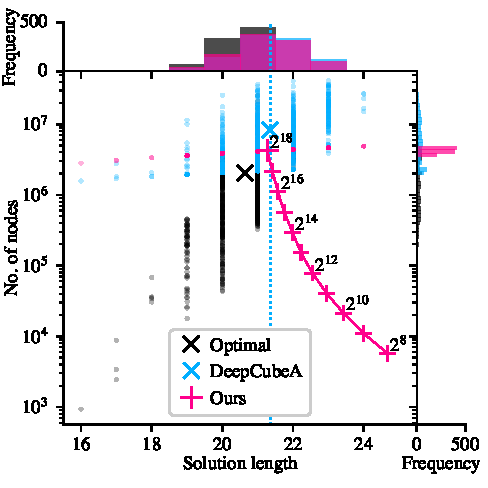
\includegraphics[width=1.0\columnwidth]{figures/results.nodes_solutions.pdf}
    \vspace{-1em}
    \caption{
        Solution length versus number of nodes on solving Rubik's Cube, by different methods.
        Each dot represents the number of moves in a solution and the number of nodes visited during a search, and we plot cross markers at their mean coordinates.
        Frequency plots are presented separately for each axis.
        The pink line indicates the trajectory of our results scaling up along the beam widths.
    }
    \label{fig:s2n}
    \vspace{-2mm}
\end{figure}


The comparison of the different methods indicates the overall advantage of our method over DeepCubeA, albeit not as powerful as the optimal solver backed by 182 GB of memory.
First, we observe that our solutions were on average shorter than DeepCubeA.
When optimal solutions averaged $20.64$ moves in length, our solutions averaged $21.27$ moves long.
Additionally, among our $1,000$ solutions, $696$ were optimal.
In both metrics of optimality, our method outperformed DeepCubeA, solutions of which averaged $21.35$ moves and were $65\%$ optimal.
Second, our solutions were also more efficient.
For training, the DNN learned the equivalent of only $1$ billion examples, while DeepCubeA did so on $10$ billion examples~\citep{agostinelli2019solving}.
When searching for solutions, DeepCubeA expanded an average of $8.19\times10^6$ nodes per solution, whereas ours expanded only $4.19\times10^6$ nodes.
These show that our method reached higher optimality than DeepCubeA, also with higher efficiencies in both training and inference.



\section{Discussion}
\begin{figure*}[t]
    \centering
    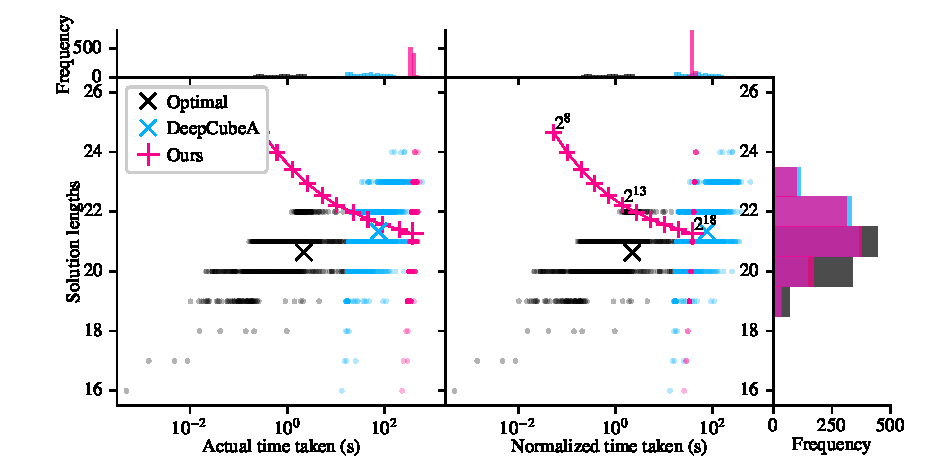
\includegraphics[width=1.0\textwidth]{figures/results.solutions_times.pdf}
    \caption{
        Calculation time versus solution length by three methods.
        The left scatterplot shows the actual time taken, and the right one shows the time normalized by per-node computation time.
        Similar to Figure~\ref{fig:s2n}, the mean coordinates are marked by a cross for all results.
    }
    \label{fig:t2s}
\end{figure*}

% Summary
Focusing on goal-predefined combinatorial problems, we proposed a novel deep learning method to directly infer the solution path.
Rather than guiding a search algorithm with distance estimation like IDA* and DeepCubeA, our method directly infers a sequence of moves leading to the goal by training a DNN merely on random scrambles.
Evaluated on solving Rubik's Cube, our method produced solutions with high optimality and efficiency, outperforming DeepCubeA on both.
The result also exhibits a smooth trade-off between compute and optimality (Figure~\ref{fig:s2n}) and a stable temporal performance (Figure~\ref{fig:t2s}).
These results suggest that our training algorithm provides stable and effective supervision signals, indirectly supporting Assumption 1 for Rubik's Cube.

% Applications
%% Limitation
Note that, as a fundamental limitation, our method requires that the target problem has a predefined goal.
For this reason, the proposed method would not directly apply to combinatorial \textit{optimization} problems like Traveling Salesman Problem, which we mentioned in Introduction, as the task is to find the optimal combinatorial state itself.
For this kind of problem, classic heuristic/approximation algorithms would remain the best approach~\citep{rego2011traveling, vanbevern2020118}, though there also are deep learning methods leveraging reinforcement learning and graph neural networks~\citep{mazyavkina2021reinforcement, joshi2022learning}.

Besides Assumption 1, because our method generates the training data backward from the goal, it also implicitly assumes the reversibility of moves.
In other words, the implicit graph of the target problem must have bidirectional edges.
If scrambles/solutions of the target problem do not follow such a reversible process, our method will not work; for example, if state transitions are non-deterministic and subject to randomness.

%% applicability

Nevertheless, under Assumption 1, our method is applicable to similar goal-predefined problems, such as 15 Puzzle and its variants, Lights Out, Sokoban, etc., which are also solved by DeepCubeA~\citep{agostinelli2019solving}.
In Appendices, we provide example applications of our method on 15 Puzzle (Appendix~\ref{appendix:15}) and on Lights Out (Appendix~\ref{appendix:lightsout}) using the same DeepCubeA dataset. Notably, our method was able to solve all of $500$ test cases of $7\times7$ Lights Out \textit{optimally}, expanding only the necessary nodes using the greedy search.


\section{Conclusion}
We presented a simple yet powerful deep learning method to solve a goal-predefined combinatorial problem like Rubik's Cube.
Through the experiment, we demonstrated that a DNN can learn to solve the target problem simply from random scrambles.
Despite the training data being random, interestingly, the resulting solutions also exhibited a high level of optimality and efficiency.
In future research, we seek to extend the proposed method with fewer constraints, e.g., to problems with a weighted graph and/or continuous space, etc.
We hope that our work provides useful perspectives on combinatorial search as well as adjacent machine learning tasks.

\section*{Code \& Data}
% Code, models, and solutions are available at:\\
We release our code, models, and experimental results at \\
\rurl{github.com/kyo-takano/EfficientCube}.

% % In the unusual situation where you want a paper to appear in the
% % references without citing it in the main text, use \nocite
% \nocite{langley00}

\bibliography{main}
\bibliographystyle{icml2022}


%%%%%%%%%%%%%%%%%%%%%%%%%%%%%%%%%%%%%%%%%%%%%%%%%%%%%%%%%%%%%%%%%%%%%%%%%%%%%%%
%%%%%%%%%%%%%%%%%%%%%%%%%%%%%%%%%%%%%%%%%%%%%%%%%%%%%%%%%%%%%%%%%%%%%%%%%%%%%%%
% APPENDIX
%%%%%%%%%%%%%%%%%%%%%%%%%%%%%%%%%%%%%%%%%%%%%%%%%%%%%%%%%%%%%%%%%%%%%%%%%%%%%%%
%%%%%%%%%%%%%%%%%%%%%%%%%%%%%%%%%%%%%%%%%%%%%%%%%%%%%%%%%%%%%%%%%%%%%%%%%%%%%%%
\newpage
\appendix
\section{Assumption 1 on \textit{2$\times$2$\times$2} Rubik's Cube}\label{appendix:mini}

We test Assumption 1 on the 2$\times$2$\times$2 version of Rubik's Cube, which has a relatively small state space ($3,674,160$ cases).
For this problem, God's Number is known to be $11$ moves in the half-turn metric, which counts both 90° and 180° turns as one move.
With one piece fixed, any state has three faces to rotate and 9 possible moves.
Accordingly, by excluding self-canceling moves (e.g., \texttt{R2} after \texttt{R'}) to reduce the number of permutations, we were able to compute all the possible scramble paths from the goal.

We aggregated frequency ranks of optimal moves (i.e., the first move of optimal paths) to all the possible states.
Since some states can have more than one optimal move, we counted for both highest- and lowest- rank optimal moves.
Figure~\ref{fig:mini} summarizes the result.
About $97.7\%$ of the states ($3,591,248$ cases) have one or more optimal moves being the most frequent of all the possible moves.
We also found a fairly strong bias in the same direction even for the least frequent optimal moves.
This observation is largely consistent with Assumption 1, providing partial support for our proposed method to work on the same class of problems.

\begin{figure}[tb]
    \centering
    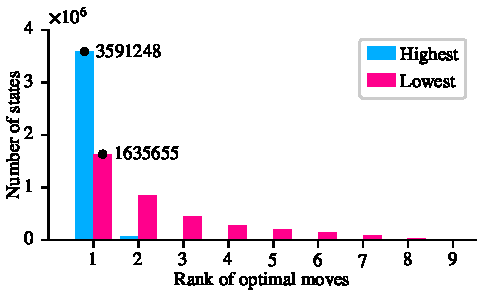
\includegraphics[width=1.0\columnwidth]{figures/appendix.mini.pdf}
    \vspace{-1em}
    \caption{Frequency distribution of nodes by highest/lowest frequency rank of optimal moves.}
    \label{fig:mini}
\end{figure}


\section{15 Puzzle}\label{appendix:15}
\begin{table*}[!t]
    \centering
    \caption{
        Performances of different methods on solving 15 Puzzle.
        Mean values are reported for solution length, number of nodes, and time taken to solve per test scramble.
        Optimal (\%) indicates the percentage of optimal solutions.
        For our and DeepCubeA's paper results, we report the calculation time normalized to the per-node temporal performance of DeepCubeA (GitHub), followed by actual time taken in parentheses.
    }
    \vspace{1em}
    \begin{tabular}{l|@{\hskip 1.5em}rr@{\hskip 1.5em}|@{\hskip 1.5em}r@{\hskip 2.0em}r@{\hskip 0.5em}c@{\hskip 1.5em}}
        \toprule
        Method                      & Solution length & Optimal (\%) & No. of nodes            & \multicolumn{2}{r}{Time taken (s)}              \\
        \midrule[0.08em]
        Optimal solver              & $52.02$         & $100.0$      & $3.22\times 10^{4}$     & $0.0019$                           &            \\
        \midrule[0.025em]
        Ours                        & $52.33$         & $84.8$       & $9.81\times 10^{6}$     & $26.42$                            & ($626.13$) \\
        \textbf{DeepCubeA (GitHub)} & \bm{$52.02$}    & \bm{$100.0$} & \bm{$3.28\times10^{6}$} & \bm{$8.82$}                        &            \\
        DeepCubeA (Paper)           & $52.03$         & $99.4$       & $3.85\times10^{6}$      & $10.37$                            & ($10.28$)  \\
        \bottomrule
    \end{tabular}
    \label{tab:result_15}
\end{table*}

\begin{figure}[!t]
    \centering
    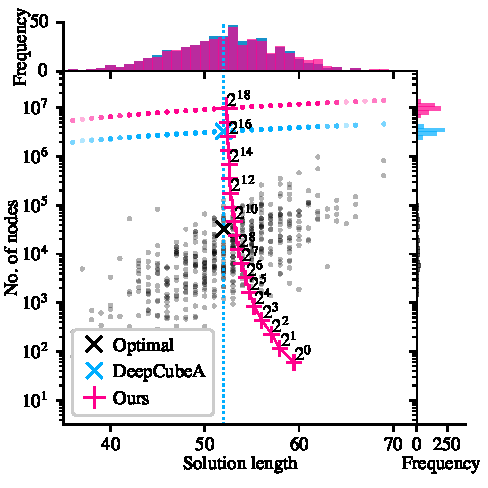
\includegraphics[width=1.0\columnwidth]{figures/appendix.15.pdf}
    \vspace{-1em}
    \caption{
        Solution length versus number of nodes on solving 15 Puzzle, by different methods.
        Each dot represents the number of moves in a solution and the number of nodes visited during a search, and we plot cross markers at their mean coordinates.
        Frequency plots are presented separately for each axis.
        The pink line indicates the trajectory of our results scaling up along the beam widths.
    }
    \label{fig:s2n15}
\end{figure}

We additionally demonstrate our method on 15 Puzzle.
15 Puzzle is a sliding puzzle consisting of 15 numbered tiles and 1 empty slot on a 4$\times$4 board.
The goal is to align the tiles in numerical order by swapping the empty slot with its neighboring tiles multiple times.
Including the goal, there are approximately $1.0\times10^{13}$ possible states, and God's Number is $80$ moves~\citep{brungger1999parallel,korf2008linear}.

We trained a DNN of the same architecture on the equivalent of $100,000,000$ solutions ($100,000$ batches $\times 1,000$ scrambles per batch) with the scramble length of $80$. Subsequently, we tested it on the same DeepCubeA dataset containing $500$ cases.
Like for Rubik's Cube, we removed obviously redundant moves like \textrightarrow{} after \textleftarrow.
On the other hand, unlike with Rubik's Cube, we sorted candidate moves by their probabilities computed through the softmax function.

Table~\ref{tab:result_15} summarizes the comparison of different models.
Figure~\ref{fig:s2n15} shows the trade-off between solution length and number of nodes.
Using the beam search, the trained DNN successfully solved all the cases with all beam widths from $2^{0}$ to $2^{18}$.
As depicted in Figure~\ref{fig:s2n15}, the resulting solutions are more optimal with increasing beam widths on average in a similar way as for Rubik's Cube.
However, contrary to DeepCubeA, our method could not always produce optimal solutions, even with more nodes expanded.
This comparative lack of success may suggest the lower degree to which 15 Puzzle satisfies Assumption 1, possibly because the number of possible moves depends on the location of the empty slot.

\section{7$\times$7 Lights Out}\label{appendix:lightsout}

\begin{table}[tb]
    \centering
    \caption{
        Performances of different methods on solving Lights Out.
        Because both DeepCubeA and our method achieved the optimal solutions across all the cases, we only report mean values of the number of nodes expanded and the \textit{actual} time taken to solve.
        We omit DeepCubeA's paper result here because both solution length and number of nodes are consistent with those of GitHub result.
    }
    \vspace{1em}
    \begin{tabular}{l|r@{\hskip 1.5em}r}
        \toprule
        Method        & No. of nodes       & Time taken (s) \\
        \midrule[0.08em]
        \textbf{Ours} & {$\bm{24.26}$}     & {$\bm{0.053}$} \\
        DeepCubeA     & $1.14\times10^{6}$ & $5.90$         \\
        \bottomrule
    \end{tabular}
    \vspace{-0.5em}
    \label{tab:result_lightsout}
\end{table}

Lights Out is a combinatorial puzzle consisting of multiple \texttt{ON}/\texttt{OFF} binary lights on a grid. In the 7$\times$7 version, 49 lights are arranged in a square.
Each light toggles the state of itself and its adjacent lights, and the goal is to turn all the lights off given a random state.
As a goal-predefined combinatorial problem, it possesses a more relaxed setting due to the following characteristics.
First, because every move is binary, using the same move twice is clearly redundant.
Also, the puzzle is commutative, meaning that the order of moves is irrelevant to the resulting state.
All moves comprising a given scramble sequence can come to the end of that sequence with equal probability.
Hence, for a DNN, the problem is a simple pattern recognition task to predict the \textit{combination} of moves, rather than specifically the last one in the permutation.
According to \citet{agostinelli2019solving}, a solution is optimal when it has no duplicate moves.

Since God's Number is unknown for this problem, we set the training scramble length to $49$ moves, the upper bound for when you need to toggle every button.
As a scramble progressed, we trained a DNN of the same architecture to predict all the moves applied to the problem up to that point.
In total, the DNN learned the equivalent of $10,000,000$ scrambles ($10,000$ batches $\times$ $1,000$ scrambles/batch).

Tested on the DeepCubeA dataset containing $500$ cases, our method successfully solved all of them \textit{optimally} with greedy search, which expands the most promising node only at every step.
Table~\ref{tab:result_lightsout} compares both our and DeepCubeA results.
Although DeepCubeA also solved all the test cases optimally, our method significantly outperformed it in terms of search efficiency, expanding nodes straight through optimal solutions.
Note, however, that this flawless result does not indicate the completeness of the trained DNN as a search heuristic.



% You can have as much text here as you want. The main body must be at most $8$ pages long.
% For the final version, one more page can be added.
% If you want, you can use an appendix like this one, even using the one-column format.
% \input{sections/Appendix} 

%%%%%%%%%%%%%%%%%%%%%%%%%%%%%%%%%%%%%%%%%%%%%%%%%%%%%%%%%%%%%%%%%%%%%%%%%%%%%%%
%%%%%%%%%%%%%%%%%%%%%%%%%%%%%%%%%%%%%%%%%%%%%%%%%%%%%%%%%%%%%%%%%%%%%%%%%%%%%%%


\end{document}


% This document was modified from the file originally made available by
% Pat Langley and Andrea Danyluk for ICML-2K. This version was created
% by Iain Murray in 2018, and modified by Alexandre Bouchard in
% 2019 and 2021 and by Csaba Szepesvari, Gang Niu and Sivan Sabato in 2022. 
% Previous contributors include Dan Roy, Lise Getoor and Tobias
% Scheffer, which was slightly modified from the 2010 version by
% Thorsten Joachims & Johannes Fuernkranz, slightly modified from the
% 2009 version by Kiri Wagstaff and Sam Roweis's 2008 version, which is
% slightly modified from Prasad Tadepalli's 2007 version which is a
% lightly changed version of the previous year's version by Andrew
% Moore, which was in turn edited from those of Kristian Kersting and
% Codrina Lauth. Alex Smola contributed to the algorithmic style files.

